\documentclass[a4paper,10pt,headlines=3.2]{scrartcl}
\usepackage{graphicx}           %Bilder

%\usepackage[T1]{fontenc}        %Umlaute
%\usepackage[latin1]{inputenc}   %Windows
%\usepackage[utf8x]{inputenc}	%Linux
\usepackage{ucs}

\usepackage[ngerman]{babel}     %Deutsche Sprache
\usepackage{amsmath}            %Math. Zeichen
\usepackage{pifont}             %Skalierbare Schriftart
\usepackage{array}
\usepackage{epsfig}             %Erweiterte Grafiken
\usepackage{makeidx}            %Stichwortverzeichnis
\usepackage[pdftex]{color} 

\newcommand{\changefont}[3]{
\fontfamily{#1} \fontseries{#2} \fontshape{#3} \selectfont}

\makeindex

\usepackage[automark]{scrpage2}
\usepackage[nosectionbib]{apacite}               %Zitieren

%\usepackage[colorlinks]{hyperref}%Hyperlinks

\usepackage{lmodern}
\usepackage{scrpage2}           %KOMA-Script
\usepackage{tipa}
\usepackage{qtree}
\usepackage{pgf}


\usepackage{remreset}			%Fussnoten global
\makeatletter
\@removefromreset{footnote}{chapter}
\makeatother 

\setcounter{tocdepth}{3}

%Kopfzeilen
\pagestyle{scrheadings}         %Seitenstil scrheadings verwenden

%\setlength{\textheight}{24cm}
%\setlength{\textwidth}{16cm}
%\setlength{\topmargin}{-2cm}
%\setlength{\oddsidemargin}{0cm}

% Groesse des Textbereiches in der Seite
\setlength{\textwidth}{16cm}
\setlength{\textheight}{22cm}
% Kopf- und Fusszeile, Hoehe und Abstand vom Text
\setlength{\headheight}{15pt}
\setlength{\headsep}{0.8cm}
% Linker Seiteneinzug
\setlength{\oddsidemargin}{2.5cm} \addtolength{\oddsidemargin}{-1in}
\setlength{\evensidemargin}{2.5cm} \addtolength{\evensidemargin}{-1in}
% Andere Groessen ausrechnen (vertikal zentrieren)
\setlength{\footskip}{\headsep}
\addtolength{\footskip}{\headheight}
\setlength{\topmargin}{\paperheight}
\addtolength{\topmargin}{-\textheight}
\addtolength{\topmargin}{-\headheight}
\addtolength{\topmargin}{-\headsep}
\addtolength{\topmargin}{-\footskip}
\addtolength{\topmargin}{-2in}
\addtolength{\topmargin}{-0.5\topmargin}

%Schriftart
\changefont{cmss}{m}{n}

%Abstand zur�cksetzen
\setlength{\headheight}{20pt}

\usepackage{listings} 
\lstset{numbers=left, numberstyle=\tiny, numbersep=5pt} \lstset{language=Java} 

\clearscrheadfoot
%\renewcommand{\headheight}{40pt} 
\ihead[]{Datenstrukturen und Algorithmen \\Fr�hlingssemester 2011 \\Institut f�r angewandte Mathematik} % - links
\ohead[asdasd]{�bung 10 \\Abgabetermin 12. Mai 2011 \\Adrianus Kleemans [07-111-693]} % - linke Kopfzeile 
\setheadsepline{.4pt} %Separate Linie im Kopf
\cfoot[\pagemark]{\pagemark} %- mittlere Fusszeile 

\begin{document}
\section*{Theoretische Aufgaben}
\subsection*{Aufgabe 1}
Gesucht: \textit{Maximale Menge paarweise zueinander kompatible Aktivit�ten}.\\
Unterste Zeile: Ganze Auswahl. Rot: (nicht optimale) Auswahl der n�chsten Aktivit�t. Gr�n: optimale Auswahl. 
\begin{figure}[ht]
\centering
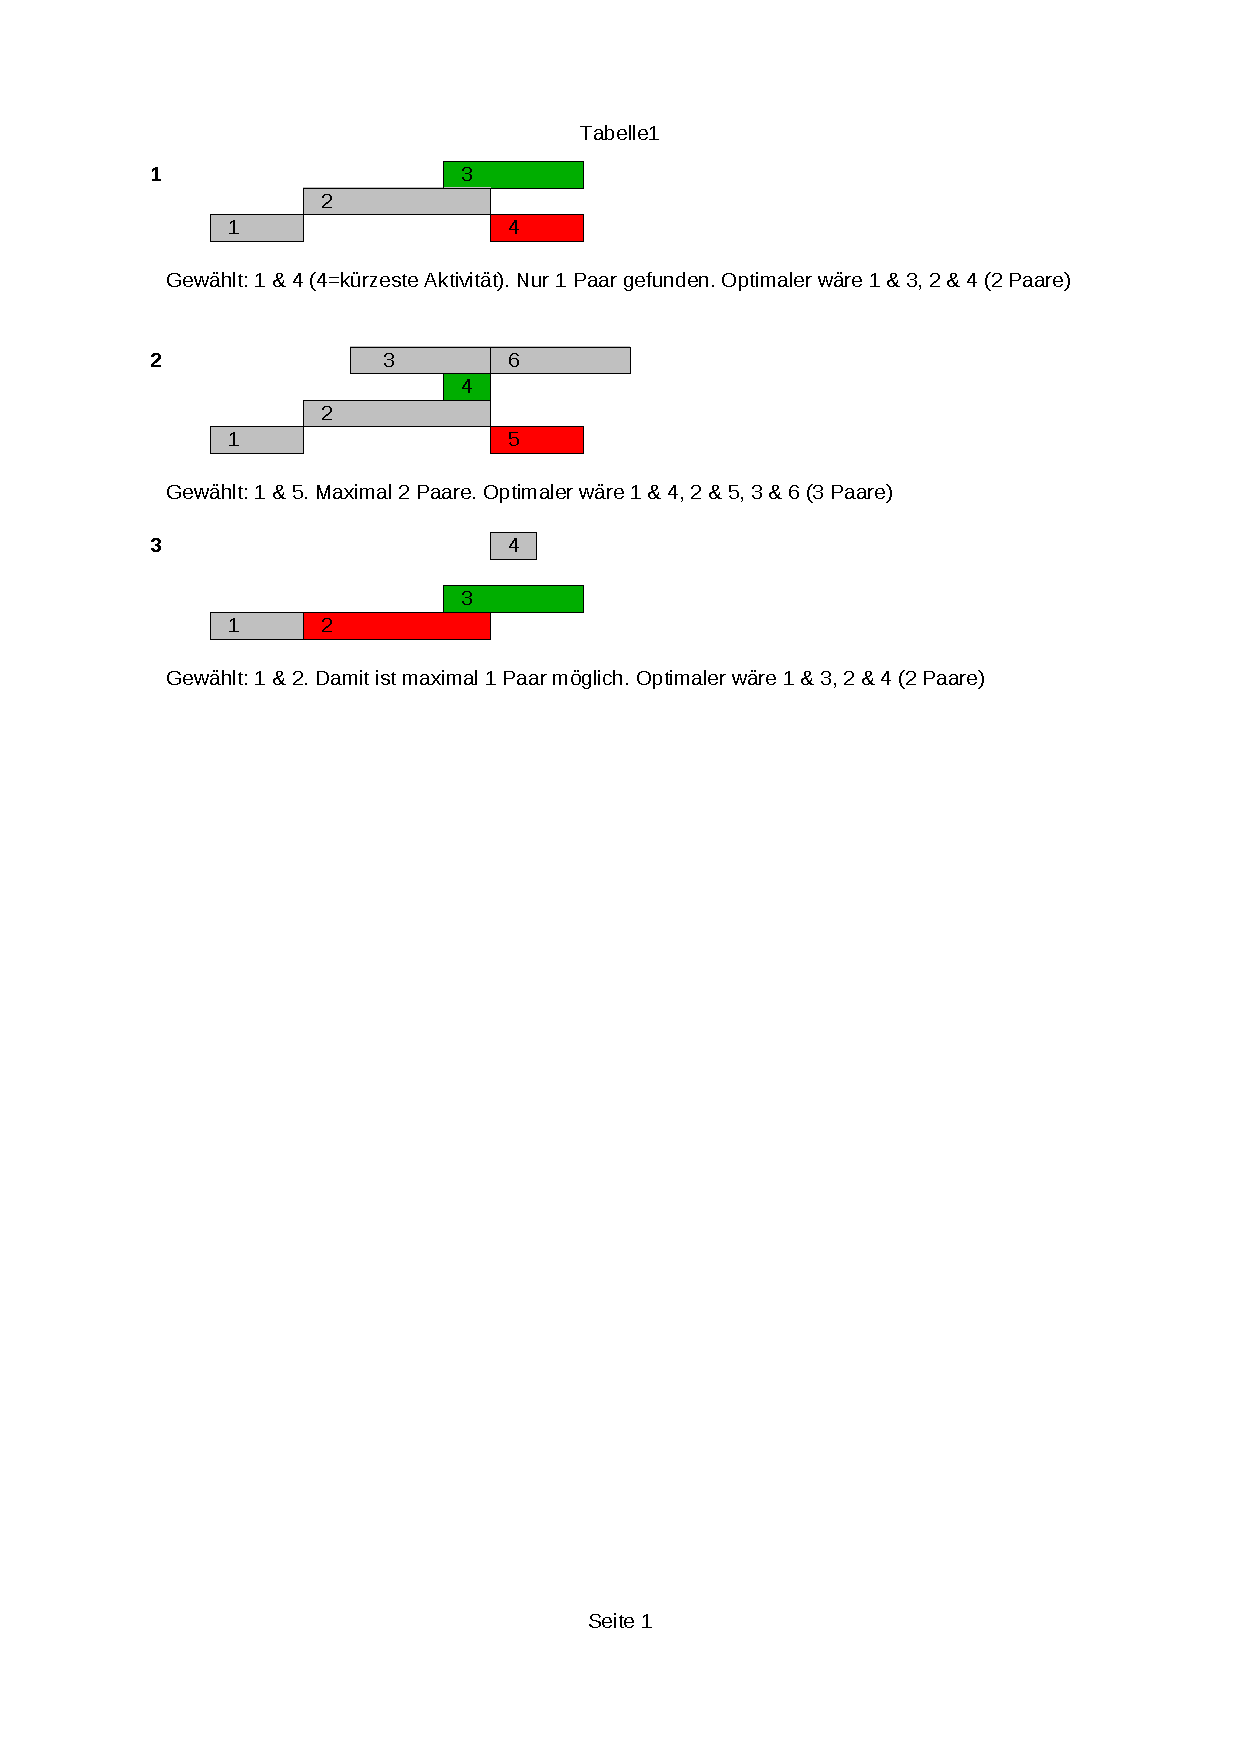
\includegraphics[height=8cm]{aufg1}
\end{figure}

\subsection*{Aufgabe 2}
H�ufigkeit: \texttt{a:4, b:6, c:1, d:2, e:1, f:3, g:1}.\\
Sortiert: \texttt{c:1, e:1, g:1, d:2, f:3, a:4, b:6}.\\
\begin{figure}[ht]
\centering
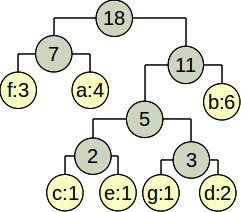
\includegraphics[height=5cm]{aufg2}
\end{figure}

\subsection*{Aufgabe 3}
\begin{itemize}
 \item a) Greedy-Algorithmus: Nimm die gr�sstm�gliche M�nze, die kleiner oder gleich gross ist wie der Gesamtbetrag.
\lstset{frame=single}
\begin{lstlisting}[caption=Aufgabe 3]{Name}
int[] chooseCoins(int n)
int[] coins = {25, 10, 5, 1}
int[] coinsChosen = {}
int moneyLeft = n

while moneyLeft > 0
   for i = 0 to coins.size
      if (coins[i] >= moneyLeft) 
         coinsChosen.add(coins[i])
         moneyLeft -= coins[i]
	 break

return coinsChosen
\end{lstlisting}
\textbf{Optimale Teilstruktur}\\
Das Wechselgeld-Problem hat in dieser Form eine optimale Teilstruktur. Wird von einem anf�nglichen Betrag \textit{n}
der bestm�gliche Betrag abgezogen, dann bleibt ein optimaler Teilbetrag, von dem wieder ein bester Betrag abgezogen
werden kann. Die Teilbetr�ge sind alle f�r sich optimal, da mit dem Greedy-Algorithmus der beste Betrag gew�hlt
wird.\\\\
\textbf{Gierige-Auswahl-Eigenschaft}\\
F�r jeden Betrag gibt es eine optimale l�sung, welche die gierige Auswahl enth�lt:\\
z.B. f�r Betr�ge ab 25 Rappen muss immer 25 Rappen enthalten sein. Wenn z.B. 40 Rappen in \{10, 10, 10, 10\} aufgeteilt
wird, kann man die Betr�ge ersetzen mit \{25, 10, 5\}, um eine verbesserte L�sung zu enthalten.\\
Beispiel f�r Nennwert 10: 12 Rappen kann in \{5, 5, 1, 1\} unterteilt werden. \{5, 5\} kann jedoch durch \{10\} ersetzt
werden (die optimale L�sung).\\
Beispiel f�r Nennwert 5: 8 Rappen kann man in \{1, 1, 1, 1, 1, 1, 1, 1\} aufteilen, aber au mit der gierigen Auswahl in
\{5, 1, 1, 1\}.\\
Beispiel f�r Nennwer 1: 2 Rappen k�nnen nur in \{1, 1\} aufgeteilt werden, welches bereits die optimale L�sung ist und
auch die gierige Auswahl enth�lt.

 \item b) Eine Menge mit \{25, 10, 1\} Rappen kann mit dem Greedy-Algorithmus zu einer suboptimalen L�sung f�hren. z.B.
30 Rappen wird in \{25, 1, 1, 1, 1, 1\} aufgeteilt, statt in optimal 3 M�nzst�cke \{10, 10, 10\}.

\begin{lstlisting}[caption=Aufgabe 3]{Name}
int[] chooseCoinsDP(int n, int[] k)
int[] denom

c[0] = 0

//loop to n (possible money values)
for j = 1 to n

   //loop through DP-table
   for i = 0 to j

      //loop through coins available
      for i2 = 0 to k.size
        if c[i]+k[i2] == j
           denom.add(k[i])
           break

return denom
\end{lstlisting}
Aufruf, um M�nzwert zu finden:
\begin{lstlisting}[caption=Aufgabe 3]{Name}
//call, denom was calculated before
int[] getCoins(int n)
int[] coinsChosen
moneyLeft = n

while moneyLeft > 0
   coinsChosen.add(denom[n])
   moneyLeft - denom[n]

return coinsChosen
\end{lstlisting}

\end{itemize}

\section*{Praktische Aufgaben}
\subsection*{Aufgabe 1, 2 & 3}
Siehe Anhang \texttt{output.txt, HuffmannCode.java} und \texttt{Node.java}.
\end{document}